\part{Soluções Apresentadas}
\chapter[Introdução]{Introdução}
Neste capítulo abordaremos todas as soluções idealizadas para o projeto. O capítulo está dividido conforme os grupos descritos na subseção ~\ref{subsec:divisao}.

\chapter[Estruturas e Materiais]{Estruturas e Materiais}

\chapter[Smart Grid]{Smart Grid}

\begin{table}[h]
  \centering
  \caption{Energia Eólica - Vantagens x Desvantagens}
  \label{my-label}
  \begin{tabular}{|l|l|}
    \hline
    \multicolumn{2}{|c|}{\textbf{Energia Eólica}}                                         \\ \hline
    \multicolumn{1}{|c|}{\textbf{Vantagens}} & \multicolumn{1}{c|}{\textbf{Desvantagens}} \\ \hline
    Energia Sustentável                      & Alto Custo                                 \\ \hline
    Energia Limpa                            & Baixa velocidade do vento na região        \\ \hline
    Energia Renovável                        & Pouca Área para instalação dos equipamento \\ \hline
  \end{tabular}
\end{table}

\begin{table}[h]
  \centering
  \caption{Energia Solar Fotovoltaica - Vantagens x Desvantagens}
  \label{my-label}
  \begin{tabular}{|l|c|}
    \hline
    \multicolumn{2}{|c|}{\textbf{Energia Solar Fotovoltaica}}                                                \\ \hline
    \multicolumn{1}{|c|}{\textbf{Vantagens}}             & \textbf{Desvantagens}                             \\ \hline
    Energia Sustentável                                  & \multicolumn{1}{l|}{Alto custo financeiro}        \\ \hline
    Energia limpa                                        & \multicolumn{1}{l|}{Geração apenas durante o dia} \\ \hline
    Simples manutenção                                   & -                                                 \\ \hline
    Alta incidência solar na região                      & -                                                 \\ \hline
    Vida útil dos painéis longa                          & -                                                 \\ \hline
    Tempo de retorno do investimento em cerca de 10 anos & -                                                 \\ \hline
  \end{tabular}
\end{table}


\begin{table}[h]
  \centering
  \caption{Gerador Movido a Biodiesel - Vantagens x Desvantagens}
  \label{my-label}
  \begin{tabular}{|c|l|}
    \hline
    \multicolumn{2}{|c|}{\textbf{Gerador Movido a Biodiesel}}                                            \\ \hline
    \textbf{Vantagens}                                      & \multicolumn{1}{c|}{\textbf{Desvantagens}} \\ \hline
    \multicolumn{1}{|l|}{Energia Sustentável}               & Alto consumo de biodiesel                  \\ \hline
    \multicolumn{1}{|l|}{Biocombustível produzido pela FGA} & Rendimento baixo                           \\ \hline
    -                                                       & Alto custo financeiro                      \\ \hline
    -                                                       & Manutenção periódica                       \\ \hline
  \end{tabular}
\end{table}


\chapter[Controle de Acesso]{Controle de Acesso}
\section{Escolha da Tecnologia}
A área de Controle de Acesso está aqui subdividida em três grandes principais frentes tecnológicas.
São elas: controle da entrada do estacionamento privativo, controle da entrada em salas e laboratórios
e, por fim, controle de frequência durante as aulas.

Dentre essas frentes, foram elegidas três possibilidades diferentes para a inserção na Universidade.
A tabela a seguir elicita-as, bem como apresenta as vantagens e desvantagens para cada um dos casos.

\begin{table}[h]
  \centering
  \caption{Tecnologias de Controle de Acesso - Vantagens x Desvantagens}
  \label{my-label}
  \begin{tabular}{|l|l|l|}
    \hline
    \multicolumn{1}{|c|}{\textbf{Tecnologia}} & \multicolumn{1}{c|}{\textbf{Vantagens}}                                                                         & \multicolumn{1}{c|}{\textbf{Desvantagens}}                                                                                                            \\ \hline
    Leitor biométrico                         & \begin{tabular}[c]{@{}l@{}}- Difícil de burlar \\ - Confiável\end{tabular}                                      & \begin{tabular}[c]{@{}l@{}}- Pode gerar falhas na leitura \\ - Não reconhecer uma \\ digital cadastrada\\ - Sistema caro\\ - Sistema frágil\end{tabular} \\ \hline
    Leitor facial/ Leitor de íris             & \begin{tabular}[c]{@{}l@{}}- Difícil de burlar \\ - Confiável\end{tabular}                                      & \begin{tabular}[c]{@{}l@{}}- Sistema de implementação\\ cara\\ - Demora para análise de \\cada pessoa\\ - Risco de furto\\ - Frágil\end{tabular}          \\ \hline
    Leitor RFID                               & \begin{tabular}[c]{@{}l@{}}- Fácil de utilizar\\ - Difícil de burlar\\ - Único para cada estudante\end{tabular} & \begin{tabular}[c]{@{}l@{}}- Custo extra para a \\faculdade\\ - Risco de perda do \\documento\end{tabular}                                                \\ \hline
  \end{tabular}
\end{table}

Apesar de todas as tecnologias sugeridas apresentarem vantagens e desvantagens, o sistema RFID foi o escolhido para atender
a demanda. Esta escolha se deu em virtude deste ser mais eficaz, eficiente e mais acessível financeiramente em relação aos
outros.

\subsection{Breve Descrição da Tecnologia RFID}
O sistema funciona RFID (do inglês \textit{Radio-Frequency IDentification}) é um tecnologia que permite identificação automática
 através de sinais de rádio. Neste projeto será implementado de  por meio de um chip dentro de um cartão, armazenando o
 nome e matrícula do aluno dono do documento e sempre que o documento for apresentado, seus dados serão apresentados nos
 display dos equipamentos. Levando em conta que tanto alunos como professores serão portadores deste documento com chip,
 para o alunos o cartão será utilizado como carteirinha, e para os professores como crachá.

Apesar de todo o grupo de controle de acesso utilizar esta ferramenta, cada uma das frentes utiliza o sistema de forma
diferente e com aparelhos diferentes. Desta forma, cada área tem suas particularidades de funcionamento e regras, como será
 mostrado e explicado a seguir.

\section{Controle de Frequência}
Para o controle de frequência nas aulas, será utilizado o seguinte aparelho (apresentado anteriormente no Ponto de Controle 1).
O funcionamento dele acontece independente de sinal de WiFi e o aparelho é de porte único do professor.

\begin{figure}[!h]
  \centering
  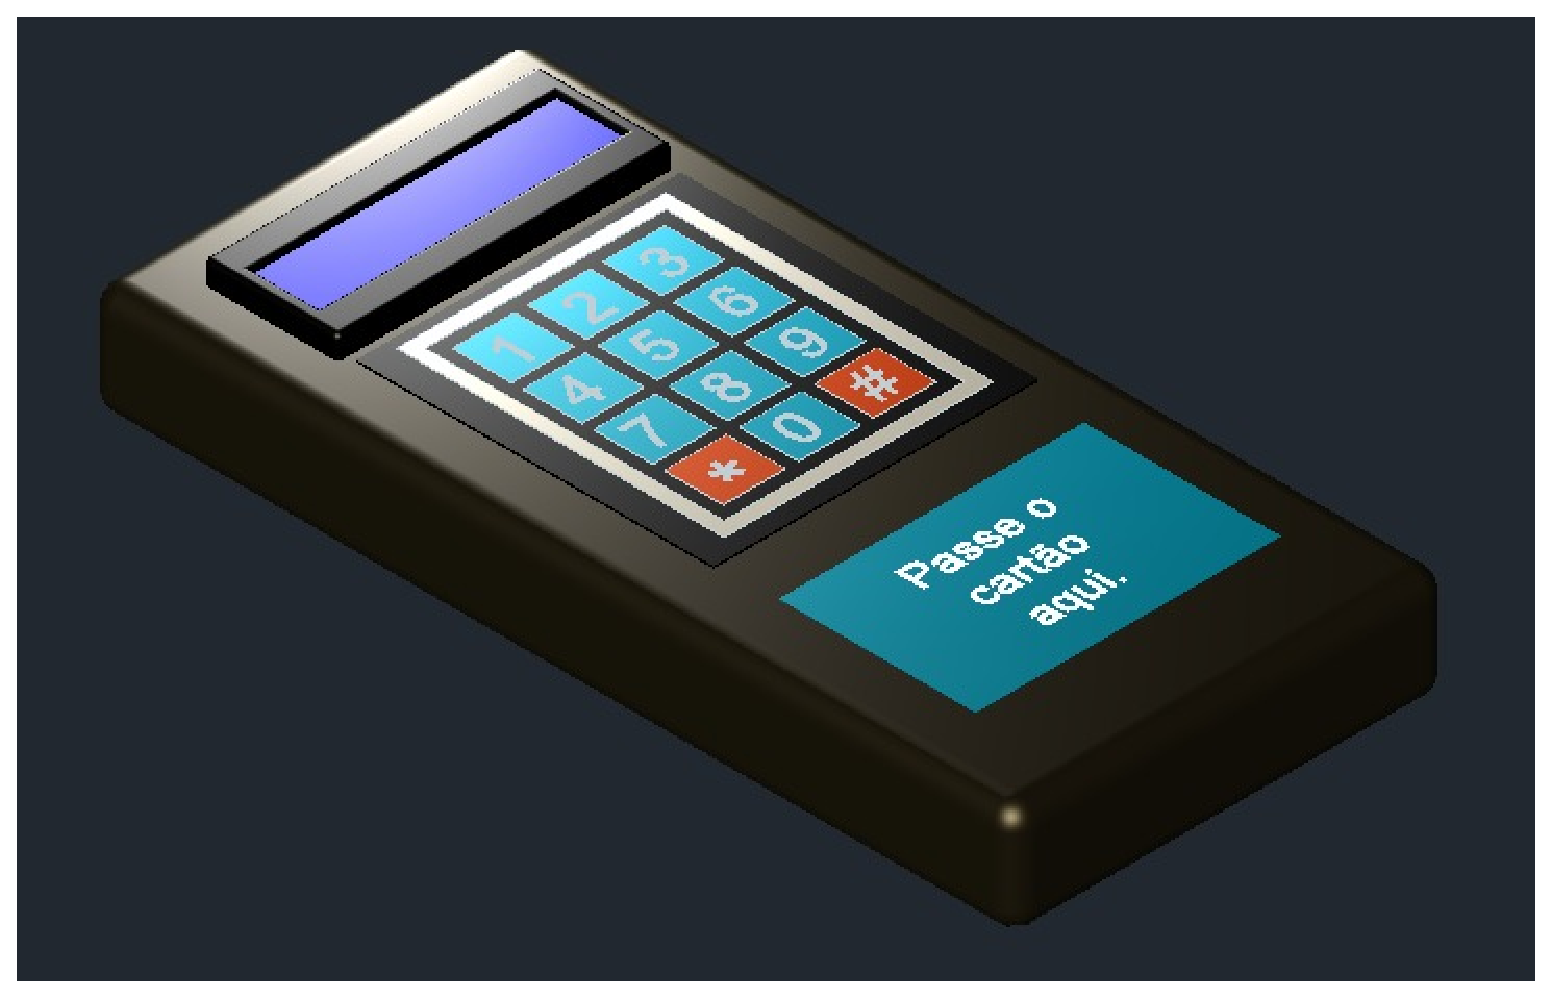
\includegraphics[keepaspectratio=true,scale=0.45]{figuras/freq.eps}
  \caption{Aparelho Para Controle de Frequência}
\end{figure}

Em relação à aspectos técnicos do aparelho, a figura a seguir mostra detalhadamente quais os instrumentos utilizados.

\begin{figure}[h]
  \centering
  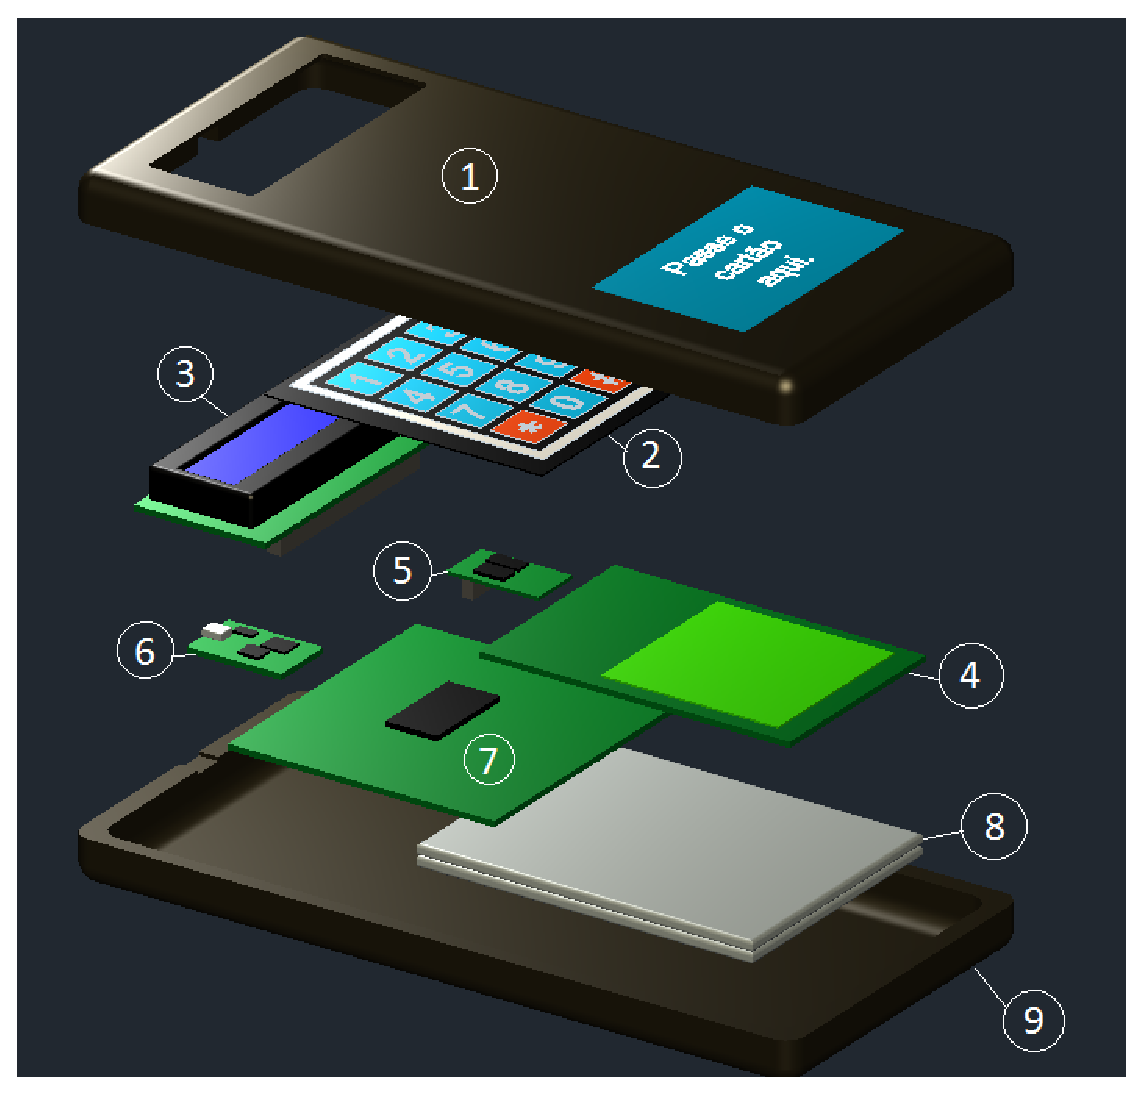
\includegraphics[keepaspectratio=true,scale=0.45]{figuras/aberto.eps}
  \caption{Aparelho Para Controle de Frequência Detalhado}
\end{figure}

Cada um dos componentes possui sua função individual:
\begin{itemize}
  \item Componentes 1 e 9: Case superior e inferior. Há um orifício na parte superior do dispositivo para passagem do conector USB.
  \item Componente 2: Teclado matricial de película 12 teclas.
  \item Componente 3: Display LCD 16x2 com backlight
  \item Componente 4: módulo Leitor de cartões RFID Mfrc522 Mifare, faz leitura e escrita em cartões RFID.
  \item Componente 5: Módulo WiFi ESP8266 ESP-01, se conecta com a rede wifi e transmite e recebe dados servidor online.
  \item Componente 6: Módulo Carregador de Baterias de Lítio TP4056, carrega a bateria através do seu conector USB.
  \item Componente 7: Placa controladora faz as conexões com os demais componentes e possui um microcontrolador ATmega1280 16au da família AVR com o bootloader do Arduino mega.
  \item Componente 8: Baterias do tablet Dl Lenoxx Navcity Phaser. Possuem capacidade de 2000mAh e tensão de 3,7v.
\end{itemize}

Cada um desses microcomponentes têm funções específicas que garantem o funcionamento adequado do instrumento. Sob uma ótica mais específica temos:

\subsection{Kit Módulo Leitor Rfid Mfrc522 Mifare}


Este módulo leitor RFID baseado no chip MFRC522 da empresa NXP é altamente utilizado em comunicação sem contato a uma frequência de 13,56MHz. Este chip, de baixo consumo e pequeno tamanho, permite sem contato ler e escrever em cartões que seguem o padrão Mifare, muito usado no mercado.

Este leitor RFID possui as ferramentas para um projeto de controle de acesso ou sistemas de segurança a um ótimo preço.

Este componentes vai ser conectado a o microcontrolador através dos pinos especiais sda(pino 44), sck(pino 20), miso(pino 22) e mosi(pino 21).

\begin{figure}[!h]
  \centering
  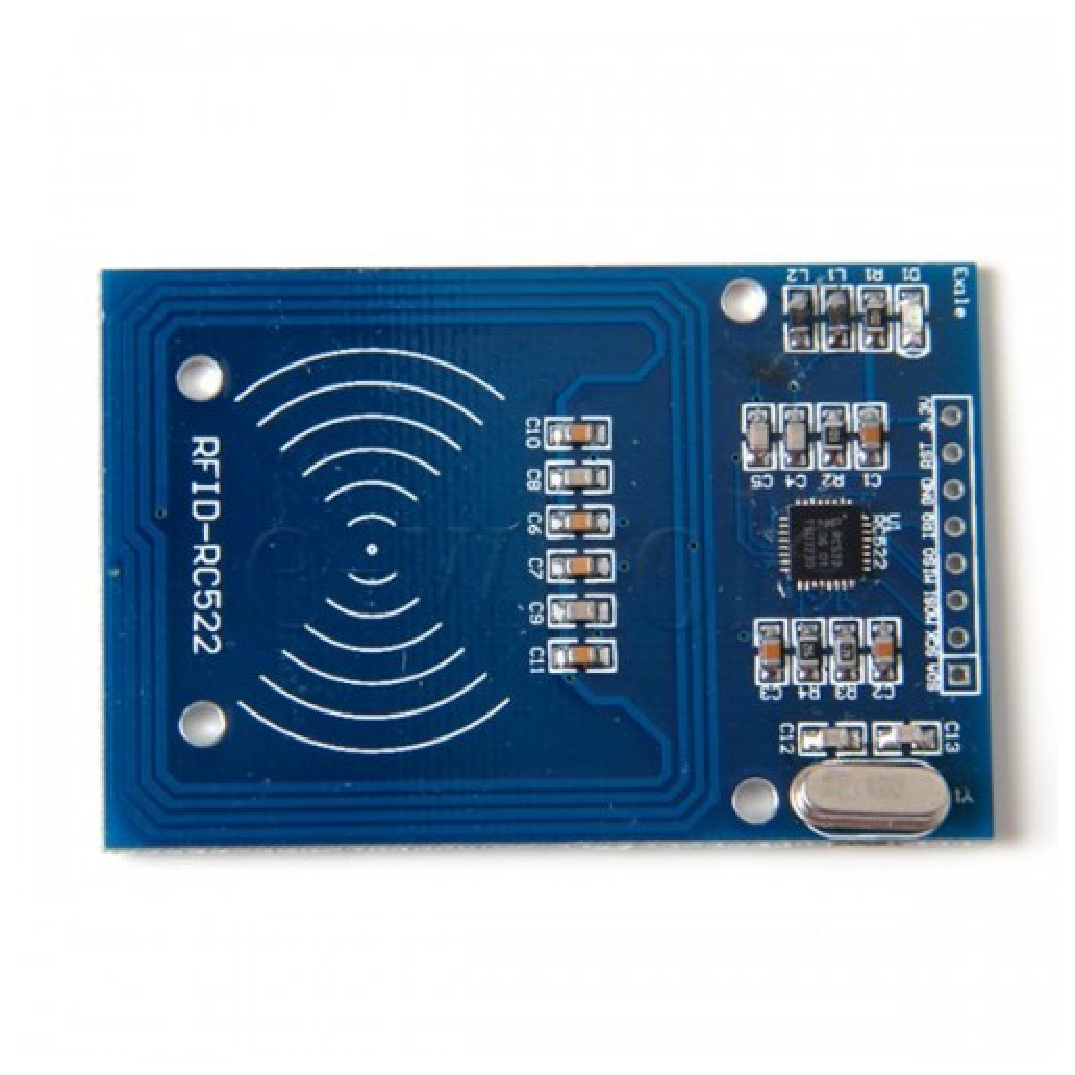
\includegraphics[keepaspectratio=true,scale=0.5]{figuras/rfid.eps}
  \caption{Módulo Leitor Rfid Mfrc522 Mifare}
\end{figure}


\subsection{Módulo WiFi ESP8266 ESP-01}
O módulo wireless ESP8266 foi desenvolvido para que seja possível conectar o microcontrolador a uma conexão WiFi de forma fácil, eficaz e a um baixo preço.

Este módulo suporta as redes 802.11 b/g/n, muito usadas atualmente, podendo trabalhar como um Ponto de Acesso (Access Point) ou como uma Estação (Station), enviando e recebendo dados.

A comunicação serial pelo protocolo RS-232, irá utilizar as portas RX(pino 45) e TX(pino 46) do microcontrolador que possuem suporte para este protocolo de comunicação TX e diretamente a protoboard. Ele será utilizado para enviar as informações coletadas pelo dispositivo ao banco de dados na rede.
\pagebreak

\begin{figure}[!h]
  \centering
  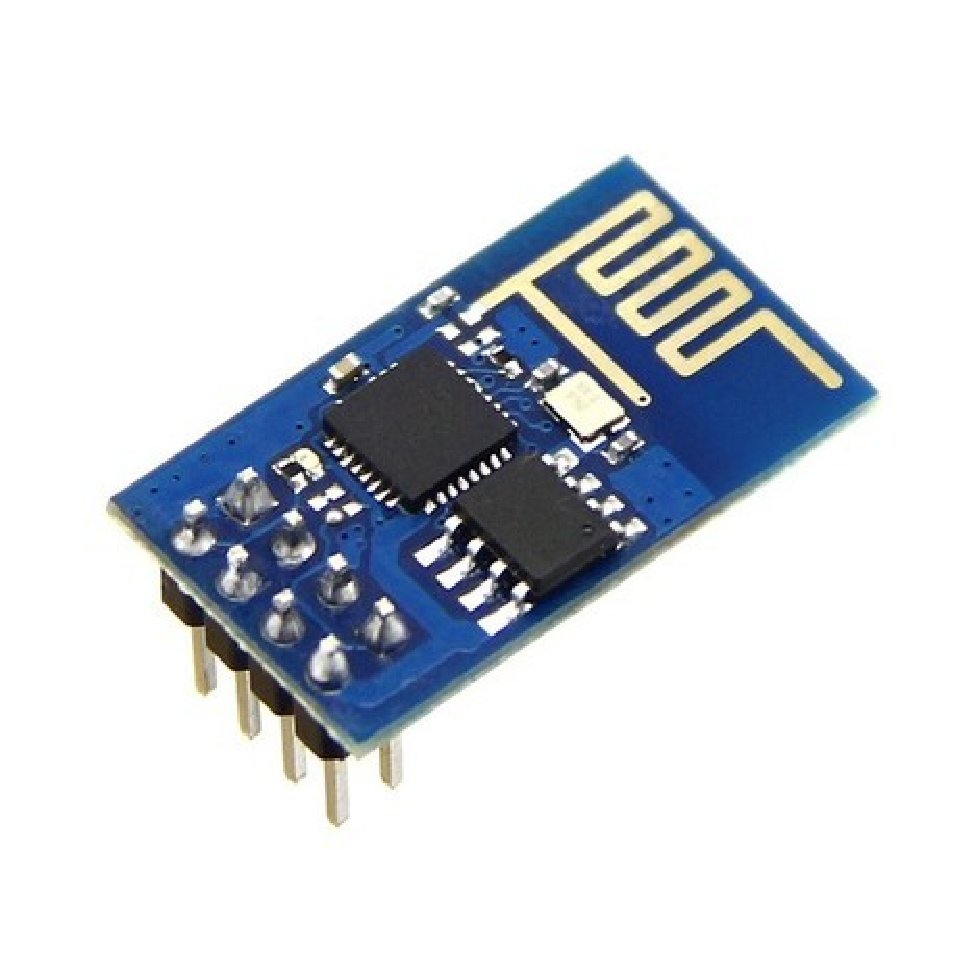
\includegraphics[keepaspectratio=true,scale=0.5]{figuras/wifi.eps}
  \caption{Módulo Leitor Rfid Mfrc522 Mifare}
\end{figure}


\subsection{Display LCD 16x2}
Este é um display LCD de 16 colunas por 2 linhas, backlight azul e escrita branca. Possui o controlador HD44780 usado em toda indústria de LCD's como base de interface.

A interface com microcontrolador é muito simples, sendo basicamente 4 pinos digitais de dados e 2 pinos digitais de controle. Confira no link o Datasheet Display LCD 16x2. O display será utilizado para mostrar a matrícula e o nome do dono da carteirinha, possibilitar ao professor selecionar a disciplina que deseja passar a chamada e outras informações que forem necessárias.

\begin{figure}[!h]
  \centering
  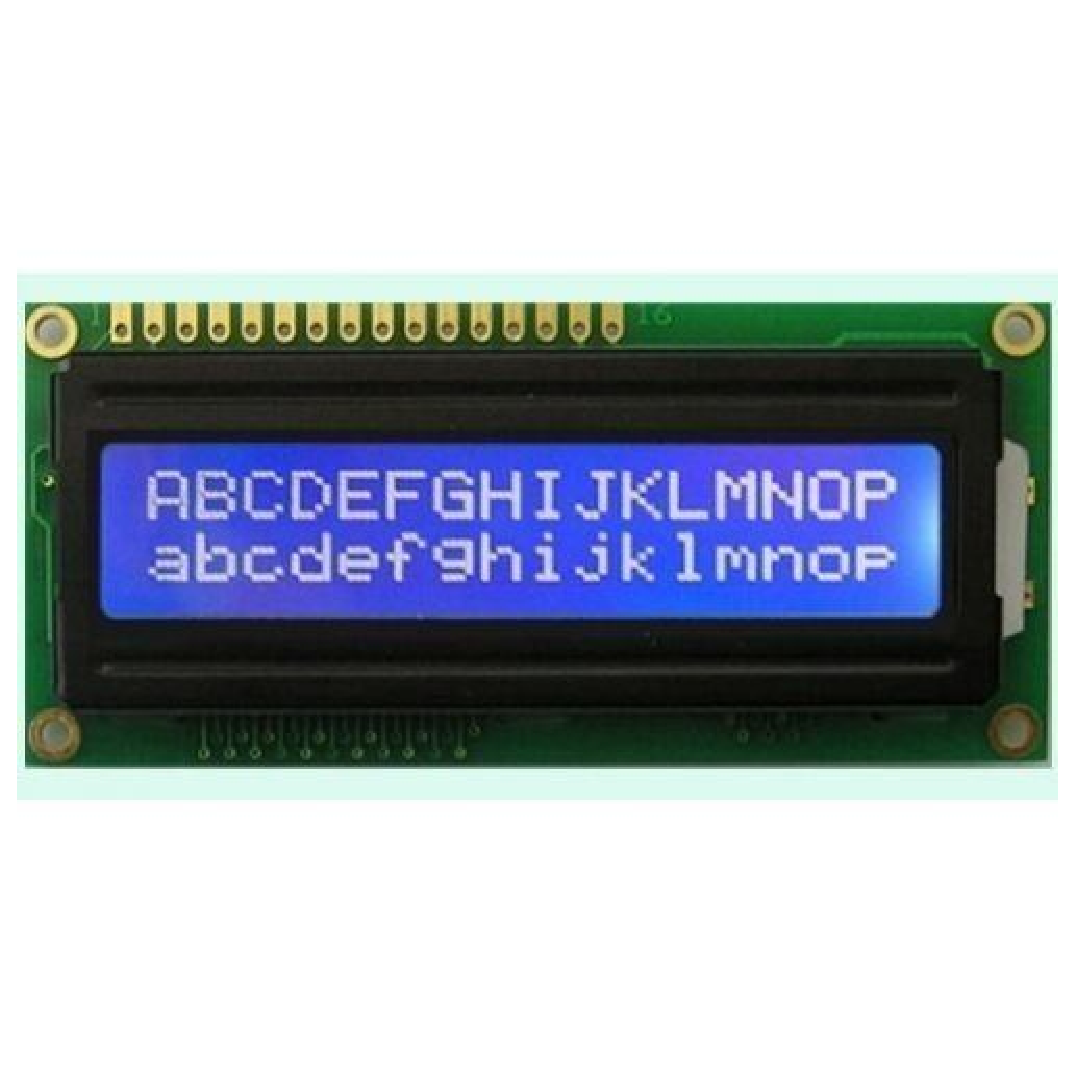
\includegraphics[keepaspectratio=true,scale=0.45]{figuras/lcd.eps}
  \caption{Display LCD}
\end{figure}

\pagebreak

\subsection{Teclado de Película 4x4}
O Teclado Matricial 4x4 é um componente utilizado para entrada de dados. Ele possui 16 teclas dispostas em 4 linhas x 4 colunas, e um conector de 8 pinos para ligação. Ele necessita de 8 pinos digitais para funcionar, sendo 4 configurados como saída(OUTPUT) e 4 como leitura(INPUT). Os pinos de saída são acionados como um contador em anel, elevando um pinos em nível alto e os demais em nível baixo, após um tempo determinado outro pino fica em nível alto e o resto em nível baixo e o ciclo se repete para cada pino. Cada pino é conectado em uma coluna da matriz e os pinos de leitura lêem as quatro linhas individualmente. Desta forma quando um botão é pressionado,  é possível determinar a linha e coluna da matriz.

\begin{figure}[!h]
  \centering
  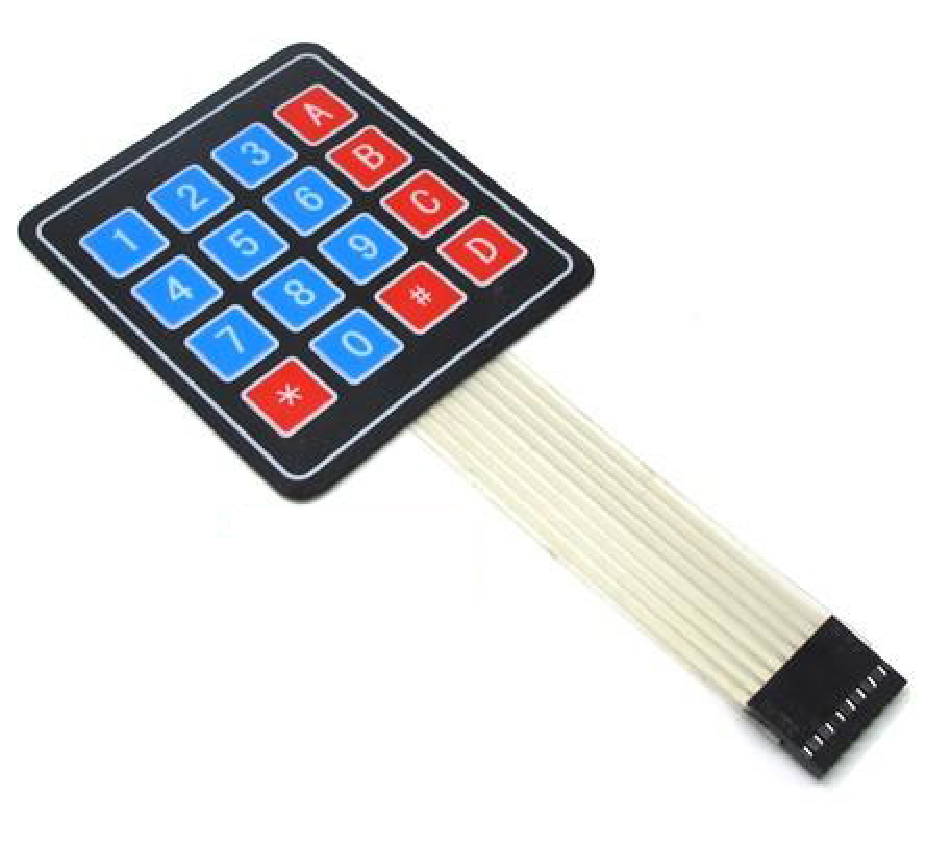
\includegraphics[keepaspectratio=true,scale=0.45]{figuras/teclado.eps}
  \caption{Teclado de Película 4x4}
\end{figure}

\subsection{Carregador de Bateria Lipo - Mini Usb TP4056}
Módulo carregador de baterias TP4056 para baterias de lítio, possibilita que as baterias sejam recarregadas sem a necessidade de removê-las do circuito. Módulo se conecta diretamente com a bateria e carrega a mesma quando é conectado um carregador USB. A corrente é cortada quando detecta que a carga está completa e possui um led indicador de carregamento. Contudo para aferir o nível de carga da bateria, será utilizado um pino analógico do microcontrolador. Medindo o nível de tensão na bateria será possível  informar o  nível de  carga através do display LCD, o que é mais prático.


\begin{figure}[!h]
  \centering
  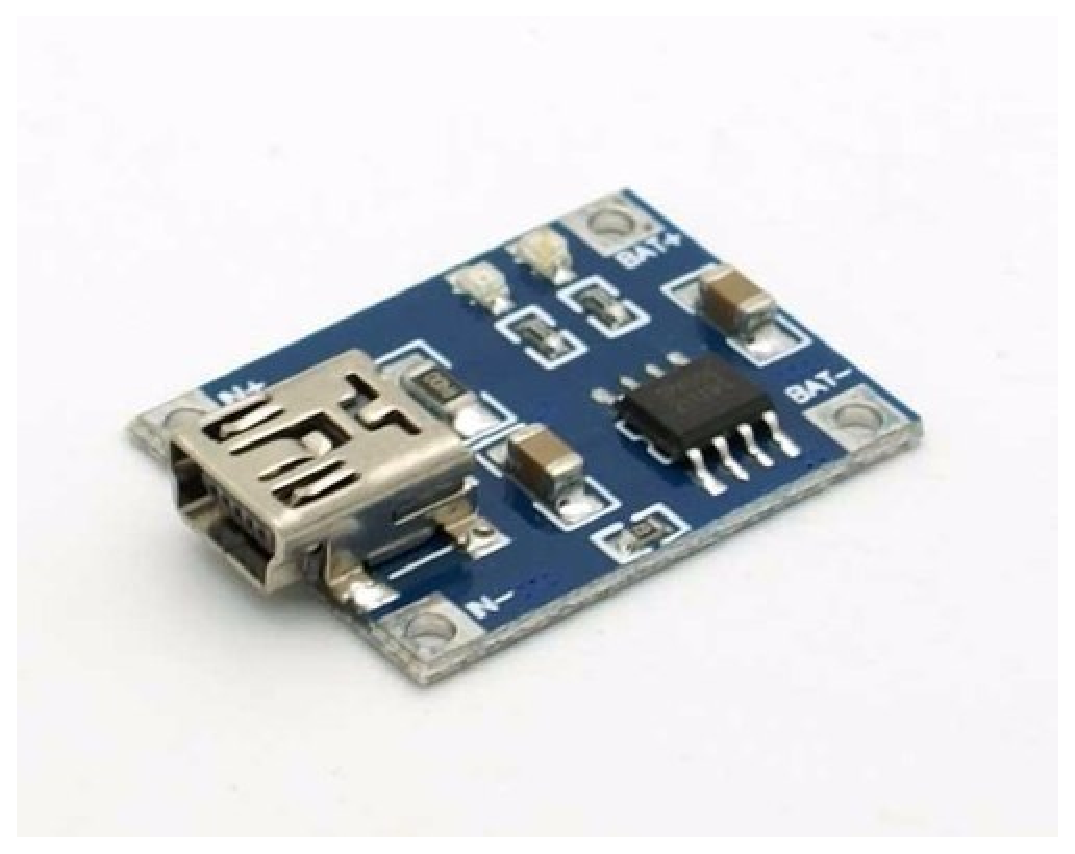
\includegraphics[keepaspectratio=true,scale=0.45]{figuras/carregador.eps}
  \caption{Carregador de Bateria Lipo}
\end{figure}

\subsection{Bateria}
Serão utilizadas duas baterias 3.7V 2000mAh em série para alimentar o dispositivo. A tensão fornecida será 7.4~6V e uma autonomia de cerca de 8 horas em uso á 157 horas (cerca de 6 dias) em \textit{standby}. Todos os componentes têm uma tensão de operação de 3.3V, apenas o display LCD opera com 5V. Para regular a tensão, será utilizado CI regulador de tensão 7805 para o display e o LM1117T para os demais.

\begin{figure}[!h]
  \centering
  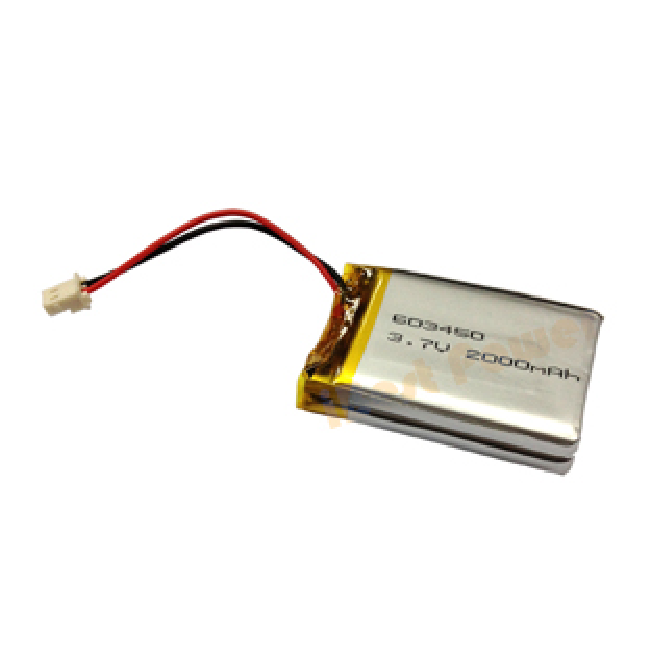
\includegraphics[keepaspectratio=true,scale=0.7]{figuras/bateria.eps}
  \caption{Bateria 2000mAh}
\end{figure}

\subsection{Microcontrolador ATmega1280}
O microcontrolador escolhido foi o ATmega1280 em função de ser o microcontrolador presente no Arduino Mega e seu número de pinos. Por isso, será possível utilizar o bootloader do arduino no microcontrolador, facilitando a programação uma vez que todos os componentes utilizados no projeto possuem bibliotecas que facilitam seu uso e implementação para arduino. Seu número de pinos digitais e especiais (TX, RX, MOSI, MISO, SDA, SCK) também foi levado em consideração durante o processo de escolha.

Em seguida, foram testados e pesquisados dados de tensão, autonomia e corrente, devido ser um aparelho portátil e de funcionamento independente da internet e sem estar ligado na tomada. Todos os dados estão apresentados na tabela a seguir.

\begin{table}[!h]
  \centering
  \caption{Dados dos Componentes - Aparelho de Frequência}
  \begin{tabular}{|l|c|c|c|}
    \hline
    \multicolumn{1}{|c|}{\textbf{Componentes}}                  & \parbox[t]{2cm}{\textbf{Corrente máxima (mA)}} & \multicolumn{1}{l|}{\parbox[t]{2cm}{\textbf{Corrente mínima (mA)}}} & \parbox[t]{5cm}{\textbf{Tensão de nominal (V)}} \\ \hline
    \parbox[t]{6cm}{Kit Módulo Leitor Rfid Mfrc522 Mifare\\}                       & 13                            & 10                                        & 3,3                            \\ \hline
    \parbox[t]{6cm}{Cartão RFID Programável Mifare 13,56Mhz}                     & -                             & -                                         & -                              \\ \hline
    Módulo WiFi ESP8266 ESP-01                                  & 215                           & 0,9                                       & 3,3                            \\ \hline
    LCD 16x2                                                    & 1,5                           & 1                                         & 5                              \\ \hline
    Teclado de película 4x3                                     & 0,3                           & 0,3                                       & 3,3                            \\ \hline
    ATmega1280                                                  & 20                            & 0,5                                       & 1,8                     \\ \hline
    \parbox[t]{6cm}{Carregador De Bateria   Lipo - Mini Usb Tp4056}                & 0                             & 0                                         & 5                              \\ \hline
    Bateria 3,7v 2000mah                                        & 0                             & 0                                         & 3,7                            \\ \hline
    \multicolumn{1}{|c|}{\textbf{TOTAL}}                        & 249,8                         & 12,7                                      & -                              \\ \hline
  \multicolumn{1}{|c|}{\parbox[t]{5cm}{\textbf{Autonomia da bateria (Horas)}}} & 8                             & 157                                       & -                              \\ \hline
  \end{tabular}
\end{table}

Com base nos dados da tabela anterior, pode-se afirmar que a autonomia da bateria do dispositivo em uso contínuo poderá ser de até 8 horas e, em standby, até 6 dias. Dado que o dispositivo poderá entrar em um modo de dormência, desabilitando o wifi, o leitor e até o próprio microcontrolador, ele poderá ter uma autonomia maior que 8 horas se entrar de forma automática neste modo enquanto aguarda uso.

Por fim, em termos econômicos, obtivemos o seguintes dados de custos:


\begin{table}[!h]
  \centering
  \caption{Custos dos Componentes - Aparelho de Frequência}
  \label{my-label}
    \begin{tabular}{|l|c|c|}
    \hline
    \multicolumn{1}{|c|}{\textbf{Componente}}    & \textbf{Custo} & \textbf{Fonte}                                                                                                \\ \hline
    \parbox[t]{7cm}{Kit Módulo Leitor Rfid Mfrc522 Mifare}        & R\$ 39,90      & \href{http://www.filipeflop.com/pd-6b883-kit-modulo-leitor-rfid-mfrc522-mifare.html}{Fonte 1}                                 \\ \hline
    \parbox[t]{7cm}{Cartão RFID Programável Mifare 13,56Mhz}      & R\$ 5,90       & \href{http://www.filipeflop.com/pd-1c240a-cartao-rfid-programavel-mifare-13-56mhz.html}{Fonte 2}                              \\ \hline
    Módulo WiFi ESP8266 ESP-01                   & R\$ 29,90      & \href{http://www.filipeflop.com/pd-1f55ad-modulo-wifi-esp8266-esp-01.html}{Fonte 3}                                           \\ \hline
    LCD 16x2                                     & R\$ 16,90      & \href{http://www.filipeflop.com/pd-6b7e4-display-lcd-16x2.html?ct=\&p=1\&s=1}{Fonte 4}                                        \\ \hline
    Teclado de película 4x3                      & R\$ 10,90      & \href{http://www.filipeflop.com/pd-218a98-teclado-matricial-de-membrana-12-teclas.html?ct=\&p=1\&s=1}{Fonte 5}                \\ \hline
    ATmega1280                                   & R\$ 60,00      & \href{http://produto.mercadolivre.com.br/MLB-831270785-lote-5-pecas-atmega1280-16au-marca-atmel-100-tqfp-atmel-\_JM}{Fonte 6} \\ \hline
    \parbox[t]{7cm}{Carregador De Bateria Lipo - Mini Usb Tp4056} & R\$ 9,90       & \href{http://www.filipeflop.com/pd-36ef09-modulo-carregador-de-baterias-de-litio-tp4056.html?ct=\&p=1\&s=1}{Fonte 7}          \\ \hline
    Bateria 3,7v 2000mah                         & R\$ 19,90      & \href{http://produto.mercadolivre.com.br/MLB-763262237-bateria-tablet-universal-dl-navcity-phaser-37v-2000mah-\_JM}{Fonte 8}  \\ \hline
\end{tabular}
\end{table}

Apesar da tabela não apresentar os preços do case superior e inferior, todo o aparelho ficaria em torno de R\$ 193,30. Este é um preço considerado acessível, considerando o tempo que o aparelho pode manter um bom funcionamento.

\section{Acesso às Salas e Laboratórios}
O controle de acesso às salas e laboratórios será um sistema único na faculdade, porém alunos e professores terão um tratamento diferenciado para a liberação de entrada nas salas. Essa diferenciação ocorre principalmente pelo fato dos ambientes possuírem equipamentos caros e pela segurança dos alunos e professores durante as aulas.

\subsection{Acesso dos Professores}
Para obterem acesso às salas, os professores terão que apresentar seu cartão no leitor RFID, que por sua vez lerá
 os arquivos guardados no chip, matrícula e nome completo do docente, e gerará o token de segurança. Assim que esses
  dados de entradas forem lidos pelo aparelho, o módulo wifi do equipamento se conectará imediatamente com a rede da
   faculdade e vai comparar os dados de entrada com os que estão no banco de dados já salvos pela UnB, e caso os
    dados estejam de acordo, a placa controladora do aparelho fará conexão com os outros micro equipamentos e a
     tranca será liberada para o acesso a sala ou laboratório. Enquanto o professor não passar novamente o cartão
      para fechar a sala, a porta ficará destrancada para a entrada dos alunos.

Caso o professor esqueça o cartão seria possível a entrada nas salas por meio de uma senha cadastrada, sendo que
 essa senha somente os professores terão acesso, e cada um dos professores terá sua senha própria. Vale ressaltar
  que o horário em que o professor inicia a abertura da sala, sempre é registrado, assim como o horário de fechamento.
   Os professores terão permissão para fazer o uso de qualquer sala ou laboratório em qualquer horário em que a universidade esteja aberta.

\subsection{Acesso dos Alunos}
Para um aluno abrir as salas com trancas será necessário que ele apresente sua carteirinha com nome e matrícula na secretaria, e lá ele receberá uma senha provisória. Isso se deve ao fato de que quando um aluno passar a carteirinha no leitor RFID e o leitor fizer todo seu processo de reconhecimento, o dispositivo reconhecerá que é um aluno tentando entrar e será solicitada uma senha para ele ter o acesso nas salas. Neste caso, o dispositivo vai registrar o horário e o tempo de uso da sala no qual o aluno se responsabilizará durante esse tempo.

Caso o aluno responsável pela sala tenha que sair, será necessário que outro aluno faça o mesmo procedimento para que a sala continue aberta, fazendo com que a responsabilidade também mude para o novo aluno cadastrado. No caso das salas de estudos, em que não terão controle de acesso, todos terão entrada livre para maior liberdade de acesso dos alunos, inclusive daqueles que não são alunos da universidade.

Para a escolha do sistema RFID no controle das salas, foi feito um balanço financeiro sobre possíveis possibilidades de marcas e compradores diferentes, como é mostrado na tabelas a seguir.

\begin{table}[h]
  \centering
  \caption{Custos - Dispositivo de Frequência}
  \begin{tabular}{l|l|}
    \cline{2-2}
    \textbf{Preço Unitário}   & \multicolumn{1}{c|}{R\$ 193,30} \\ \cline{2-2}
    \textbf{TOTAL (20 salas)} & R\$ 3.866,00                    \\ \cline{2-2}
  \end{tabular}
\end{table}

\begin{table}[h]
  \centering
  \caption{Custos - Fechaduras}
  \label{my-label}
  \begin{tabular}{|l|l|c|l|c|l|}
    \hline
    \multicolumn{2}{|c|}{\parbox[t]{3cm}{\textbf{INTELBRAS FFX 1000}}} & \multicolumn{2}{c|}{\textbf{C90 HDL}}       & \multicolumn{2}{c|}{\parbox[t]{3cm}{\textbf{PROTECTION PT-710}}} \\ \hline
    \textbf{Loja}                 & \textbf{Preço}    & \textbf{Loja}              & \textbf{Preço} & \textbf{Loja}                & \textbf{Preço}   \\ \hline
    \parbox[t]{2cm}{MAGAZINE LUIZA}                & R\$ 143,91        & AMERICANAS                 & R\$ 165,90     & \parbox[t]{2cm}{PROTECTION STORE}             & R\$ 219,00       \\ \hline
    WALMART                       & R\$ 145,00        & WALMART                    & R\$ 169,00     & WALMART                      & R\$ 131,00       \\ \hline
    MERCADO LIVRE                 & R\$ 145,90        & \parbox[t]{2cm}{MERCADO LIVRE}              & R\$ 149,90     & \parbox[t]{2cm}{MERCADO LIVRE}                & R\$ 125,00       \\ \hline
    SUBMARINO                     & R\$ 145,90        & SUBMARINO                  & R\$ 179,90     & -                            & -                \\ \hline
    \parbox[t]{2cm}{RICARDO ELETRO}                 & R\$ 180,40        & \parbox[t]{2cm}{LEROY MERLIN}               & R\$ 179,90     & -                            & -                \\ \hline
    \textbf{MÉDIA:}               & R\$ 152,22        & \textbf{MÉDIA:}            & R\$ 168,92     & \textbf{MÉDIA:}              & R\$ 168,92       \\ \hline
    \parbox[t]{2cm}{\textbf{TOTAL (20 SALAS):}}    & R\$ 3.044,44      & \parbox[t]{2cm}{\textbf{TOTAL (20 SALAS):}} & R\$ 3.378,40   & \parbox[t]{2cm}{\textbf{TOTAL (20 SALAS):}}   & R\$ 3.166,67     \\ \hline
  \end{tabular}
\end{table}

A primeira tabela se refere ao dispositivo utilizado que é o mesmo do controle de frequência, já mencionado anteriormente com mais detalhes. A segunda tabela, por sua vez, mostra um detalhamento sobre os tipos de fechadura visto por empresas diferentes. Analisando toda a tabela, é notável que a fechadura Intelbras FFX 1000 tem um preço mais acessível, comparado às outras, além de ser tão eficiente quanto todas pesquisadas.

\section{Acesso ao Estacionamento}

Já foram apresentadas anteriormente (no Ponto de Controle 1) as vantagens e desvantagens do controle do acesso ao estacionamento. Em resumo: por um lado temos a sonhada segurança no campus da FGA e por outro lado temos a rejeição do público alvo com o novo sistema.

O sistema funcionará utilizando um leitor RFID de baixa frequência, essa gama de frequências estende-se dos 30KHz aos 300KHz. Os leitores, nesta gama de frequências, operam a 125 ou 135 KHz e possuem um alcance inferior a meio metro com a velocidade de transferência inferior a 1 kbits/s, o que significa que este opera em baixa interferência com o meio ambiente e tem um comportamento bom na leitura de tags em objetos contendo líquidos e metais, assim todo o processo do microcontrolador de chegar no banco de dados as informações do aluno, professor ou funcionário acontecerá, e permitirá ou não a passagem do carro para o estacionamento privativo.

Além de contar com o aparelho leitor RFID e a cancela para controlar o acesso, o estacionamento também terá uma câmera que filmará em tempo real a placa do carro e o motorista, constatando o horário de saída e entrada do carro.

Apesar desse sistema de segurança ser primordial no projeto, ele é um sistema de fácil implementação e uso, tendo em vista que não há um diferenciamento específico de pessoas que entram no estacionamento. Qualquer pessoa da faculdade pode entrar sem exceções e o sistema de banco de dados com nome e matrícula é o mesmo que outras partes de controle de acesso também utilizam.

Em termos financeiros, o projeto de controle de acesso ao estacionamento é considerado viável devido ao \textit{payback} de todos os equipamentos utilizados com é mostrado na tabela a seguir.

\pagebreak

\begin{table}[h]
  \centering
  \caption{Custos - Estacionamento}
  \begin{tabular}{|l|l|l|l|l|l|l|}
    \hline
    \multicolumn{2}{|c|}{\textbf{Item}} & \multicolumn{2}{c|}{\textbf{Quantidade}} & \multicolumn{1}{c|}{\textbf{Descrição}}                                                               & \textbf{R\$ (unidade)} & \textbf{R\$ (total)} \\ \hline
    \multicolumn{2}{|l|}{1}             & \multicolumn{2}{l|}{2}                   & \parbox[t]{6cm}{Instalação de CPU ou totens de leitura de tags RFID.}                                                  & R\$678,00              & R\$1.356,00          \\ \hline
    \multicolumn{2}{|l|}{2}             & \multicolumn{2}{l|}{2}                   & Hardware de comunicação com cancelas.                                                                 & R\$800,00              & R\$1.600,00          \\ \hline
    \multicolumn{2}{|l|}{3}             & \multicolumn{2}{l|}{2}                   & \parbox[t]{6cm}{Sensores de leitura infra-vermelho, para identificação da saida de veiculos e fechamento de cancelas.} & R\$1.200,00            & R\$2.400,00          \\ \hline
    \multicolumn{6}{|l|}{\textbf{TOTAL:}}                                                                                                                                                                           & R\$5.356,00          \\ \hline
  \end{tabular}
\end{table}

Apesar de serem equipamentos caros, estes possuem uma longa vida útil, se usados corretamente, ou seja, se trata de um investimento à longo prazo de um bem útil à todo o corpo universitário.



Vale a pena ressaltar que o aparelho de frequência é o mesmo utilizado em todas as frentes de controle de acesso, a única diferença entres as frentes é que para o controle nas salas e controle do estacionamento ele estará preso em uma superfície plana na vertical, para que o usuário possa fazer uso dele tanto em pé quanto dentro do automóvel.

\chapter[Instrumentação e Controle]{Instrumentação e Controle}

\section{Ambientação da Sala}
\subsection{Iluminação}

Nas salas de aula serão utilizadas um modelo de lâmpada inteligente que possui sensores de luminosidade e de presença. Este equipamento é capaz de ajustar a intensidade luminosa do ambiente, permitindo a manutenção automática do nível adequado de luz. A curto prazo, essa solução se apresenta um custo elevado, pois cada kit (2 lâmpadas e 1 controlador) custa cerca de R\$ 500,00. Porém, a longo prazo, possui maior custo benefício, pois apresentam uma vida útil de aproximadamente 30 anos. A lâmpada chega a consumir 60\% a 80\% (de 598,4 W/H a  1196,8 W/H) do consumo de energia elétrica comparada a uma lâmpada LED tradicional (cerca de 2992 W/H).

\subsection{Persianas Inteligentes}

Persianas automatizadas serão utilizadas para o controle de iluminação natural nos ambientes do prédio. Estas persianas são feitas de um material resistente, e podem serão instaladas na parte interna das salas. O espaçamento entre cada haste pode ser regulado, para limitar a quantidade de luz natural que entra na sala. Além disso, a fabricação das persianas impede a entrada de poeira, reduzindo os problemas que ela causa, e quando totalmente fechadas, fornecem isolamento acústico.
As persianas são controladas a partir de um mesmo ponto, simplificando e diminuindo a movimentação para abrí-las ou fechá-las dentro da sala. Seu custo médio é de R\$ 450,00.

\subsection{Sistema de Som}

Para a sonorização do ambiente da sala de aula, serão utilizadas caixas de som in-wall, com potência máxima de 160 Watts e armação reforçada de fibra de vidro. O custo é de aproximadamente R\$570,00 o par.
Para os microfones, serão utilizados dispositivos sem fio e com apoio na orelha, comodidade para o professor. O preço varia bastante, sendo encontrados valores por volta de R\$ 150,00.

\subsection{Climatização}

Serão utilizados ar-condicionados do tipo split inverter, o qual o compressor nunca desliga, então não ocorre picos de energia. Além disso, esse compressor tem a velocidade de rotação variável, se auto-regulando de acordo com a temperatura interior. Apresentam um maior custo, porém, economizam energia ao longo do tempo, o que traz benefícios.
Para as salas de aula menores, serão utilizados aparelhos com 12.000 BTUs de potência, que custa em torno de R\$1.200,00. Pela tabela do Procel o ar-condicionado de 12.000 BTUs split consume aproximadamente 193,76 KW/h.
Para as salas maiores, serão utilizados ar-condicionados mais potentes, devido a grande quantidade de alunos nas aulas e o tamanho das salas. Estes equipamentos terão 58000 BTUs de potência, que custam R\$5000,00 e pela tabela de do Procel ele consome cerca de 679,20 KW/h de energia elétrica.

\begin{table}[!h]
  \centering
  \caption{Soluções de Ambientação da Sala}
  \label{my-label}
    \begin{tabular}{|l|l|l|l|l|l|}
    \hline
    \textbf{Equipamentos} & \textbf{Descrição} & \textbf{Vantagens} & \textbf{Desvantagens} & \textbf{Consumo} & \textbf{Custo} \\ \hline
    \parbox[t]{3cm}{Lâmpada Inteligente} & \parbox[t]{2cm}{Lâmpada inteligente que possui sensores de luminosidade e de presença.} & \parbox[t]{3cm}{Economia de energia, longa durabilidade e sensores de nível de luz.} & \parbox[t]{3cm}{Custo comparado com as outras lâmpadas.} & \parbox[t]{2cm}{Entre 1196,8W/H e 598,4WH.} & \parbox[t]{2cm}{R\$560,00} \\ \hline
    \parbox[t]{3cm}{Persianas Automatizadas} & \parbox[t]{2cm}{Persianas automatizadas que funciona a partir de um determinado aplicativo.} & \parbox[t]{3cm}{Facilidade na hora de escolher abertura da persiana.} & \begin{tabular}[c]{@{}l@{}}\parbox[t]{3cm}{Falta de energia do prédio compromete o funcionamento}\\ \parbox[t]{3cm}{Custo comparado com uma persiana normal.}\end{tabular} & \parbox[t]{2cm}{Não foi encontrado.} & \parbox[t]{2cm}{R\$450,00} \\ \hline
    \parbox[t]{3cm}{Alto-Falantes} & \parbox[t]{2cm}{Caixas de som que são fixadas na parede.} & \parbox[t]{3cm}{Melhor propagação do som pela sala.} & \parbox[t]{3cm}{Falta de energia compromete o uso, e se tiver problemas de funcionamento compromete o som da sala.} & \parbox[t]{2cm}{160 Watts.} & \parbox[t]{2cm}{R\$570,00 o par.} \\ \hline
    \parbox[t]{3cm}{Microfones} & \parbox[t]{2cm}{Aparelho que converte ondas sonoras em sinais elétricos.} & \parbox[t]{3cm}{Aumento da voz do professor e melhora a qualidade de som das aulas.} & \parbox[t]{3cm}{Falta de energia compromete o uso e se tiver problemas de funcionamento pode prejudicar a qualidade do som durante as aulas.} & \parbox[t]{2cm}{12 Watts.} & \parbox[t]{2cm}{R\$ 150,00} \\ \hline
    \parbox[t]{3cm}{Ar-condicionado} & \parbox[t]{2cm}{Aparelho que regula o aquecimento ou a refrigeração do ambiente.} & \parbox[t]{3cm}{Monitoramento da temperatura do ambiente e melhora o clima da sala principalmente em épocas de calor.} & \parbox[t]{3cm}{Custo e alto gasto de energia ainda mais nas salas grandes.} & \parbox[t]{2cm}{193,76 KW/h a 679,20KW/h} & \parbox[t]{2cm}{R\$1.298,0 a R\$5449,00} \\ \hline
  \end{tabular}
\end{table}

\section{Digitalização e Integração de Equipamentos para Aula}

\subsection{Mesa Inteligente}

A mesa inteligente consiste em uma tela sensível ao toque, em formato de mesa, que permitirá que o professor controle os diversos dispositivos presentes na sala.
As características de cada dispositivo varia de um fabricante para outro, como por exemplo o tamanho da tela sensível ao toque, sendo encontradas usualmente telas de 32 a 65 polegadas, ou a presença de tecnologias de reconhecimento de objetos colocados sobre sua superfície. 
As mesas interativas possuem suporte para diferentes sistemas operacionais, como Windows, Linux, MacOs X, e até Android, o que permite a fácil integração com outros dispositivos como projetores e roteadores de internet. Isto pode possibilitar ao professor o acesso a materiais disponíveis online durante a aula, facilidade de exibição de apresentações em slides entre outras inúmeras possibilidades de uso, além de possuir um controle centralizado de todas as funções automatizadas presentes na sala de aula.

\subsection{Quadro interativo}

Além dos quadros convencionais, um quadro interativo será utilizado para auxiliar o professor, tornando as aulas expositivas mais dinâmicas. Atualmente existem diversos fabricantes de quadros interativos, com diferentes tamanhos e funcionalidades, incluindo até, em alguns casos, suites de softwares específicos para aquele determinado produto. Os dispositivos possuem diversas opções de conectividade, possibilitando a interação com computadores pessoais, dispositivos mobile e até mesmo com a mesa inteligente do professor. O custo deste equipamento varia entre R\$4.000,00 e R\$8.000,00.

\begin{table}[!h]
  \centering
  \caption{Soluções de Digitalização e Integração de Equipamentos para Aula}
  \label{my-label}
  \begin{tabular}{|l|l|l|l|l|l|}
    \hline
    \textbf{Equipamentos} & \textbf{Descrição} & \textbf{Vantagens} & \textbf{Desvantagens} & \textbf{Consumo} & \textbf{Custo} \\ \hline
    \parbox[t]{3cm}{Mesa inteligente} & \parbox[t]{2cm}{Painel de controle da sala e também um computador de uso do professor}. & \parbox[t]{3cm}{Auxilia no monitoramento do professor em relação a sala e além de ser um instrumento a mais de uso para as aulas dos professores e na aprendizagem dos alunos.} & \parbox[t]{3cm}{Alto custo e se for danificado pode comprometer as aulas dos professores e do funcionamento da sala.} & \parbox[t]{2cm}{Não encontrado.} & \parbox[t]{2cm}{\$8000,00 (Dólares)} \\ \hline
    \parbox[t]{3cm}{Quadro interativo} & \parbox[t]{2cm}{Superfície que,reconhece a escrita electronicamente e que necessita de um computador para funcionar.} & \parbox[t]{3cm}{Aumento na produtividade e exposição do conteúdo das aulas e além de ser mais uma ferramenta útil para os professores.} & \parbox[t]{3cm}{Alto custo e restrito ao local.} & \parbox[t]{2cm}{0,5W} & \parbox[t]{2cm}{Entre R\$4.000,00 e R\$8.000,00} \\ \hline
  \end{tabular}
\end{table}

\section{Status da Sala}

\subsection{Painel informativo}

A melhor solução para o painel informativo seria um display de LCD embutido na parede, onde as informações sobre o status da sala serão exibidas. Estas informações seriam enviadas em tempo real, permitindo que imprevistos ou informações de última hora sejam informadas aos usuários da sala com maior efetividade. O custo deste tipo de equipamento varia em torno de R\$300,00 e R\$1500,00, dependendo da marca e do tamanho da tela.

\section{Sensores}

\subsection{Termopar}

Os termopares medem a temperatura do ambiente utilizando-se de dois condutores metálicos diferentes unidos na mesma extremidade. Esse dispositivo funciona pelo princípio de que essa configuração citada, gera uma força eletromotriz em função dos metais e das temperaturas T1 (junta de medida) e T2 (junta de referência). Assim criou-se uma tabela de correlação entre a FEM e a função de temperatura, considerando T2=0. Para o nosso projeto, foi escolhido o termopar tipo K que é de uso genérico, tem baixo custo e mede temperaturas entre -200 e 1200C, tendo uma sensibilidade de aproximadamente 41uV/C. O custo de um termopar é de aproximadamente R\$40,00.

\subsection{Termostato}

É o dispositivo utilizado para manter a temperatura constante, composto por um sensor que mostra a variação de temperatura e um que controla essa variação. Aqui pode se aplicar o Ecobee 3 que custa \$169. Esse aparelho possui um sensor de movimento, priorizando sua utilização onde detecta movimento e ainda mantém a tela em modo de economia de energia até detectar que alguém está se aproximando da tela. Ele funciona via Wi-fi e aplicativos, além do que pode se conectar a mesa inteligente.

\subsection{Sensores de Calor}

Será usado como sensor de calor o detector de temperatura e Fumaça Combinados, código AFVRFTH da empresa ABAFIRE. É um equipamento que deve ser instalado no teto ou na parede das edificações e tem como função enviar um alerta para uma Central de Alarme de Incêndio assim que detecta o aumento brusco da temperatura ambiente ou a presença de fumaça. Este alerta serve para avisar ao responsável pela segurança da edificação que, possivelmente, existe uma situação emergencial no local, como um princípio de incêndio . O sensor consegue identificar pela elevação da temperatura quanto pela presença de fumaça.Ele detecta a partir dos 55C e tem uma cobertura circular de 4,2 metros. É alimentado com 24V .Possui LED vermelhos de vigília e alarme.Consumo de 30 uA em repouso e 30MA quando é ativado. O sensor estaria interligado com a sala de controle para que seja avisado o perigo de incêndio no local e ele se encontra no mercado entre R\$150 e R\$ 250. 

\subsection{Sensor de movimento}

O sensor de movimento será utilizado para o controle de luz do ambiente, fazendo com que não tenha desperdício de energia ao deixar as luzes ligadas. Esse sensor seria basicamente para, no caso de deixarem a luz ligada, depois de um certo tempo e verificando que não tem ninguém no local, as luzes sejam apagadas automaticamente. O preço dos sensores varia, tendo sensores que custam R\$15,00 (no caso, seria apenas o sensor, tendo que fazer o circuito para o funcionamento do mesmo) e sensores prontos para uso, que variam o preço entre R\$35,00 e R\$ 210,00.

\subsection{Fototransistores}

Dispositivo utilizado na lâmpada responsiva, que variam a resistência elétrica de acordo com a intensidade luminosa do local. Ele possui dois diodos de junção, o coletor e o emissor; a base é incluída quando tem-se polarização ou controle elétrico. Quando recebem fótons, o conjunto base-coletor cria lacunas na sua vizinhança e a tensão faz com que as lacunas sejam transmitidas para o emissor. Enquanto isso os elétrons do emissor sao tranferidos para a base, aumentando a corrente nela e, consequentemente, variando a corrente no coletor. Assim, com a base desconectada, a corrente dependerá da intensidade luminosa incidente. Um fototransistor 3mm custa em média R\$5,00.

\begin{table}[!h]
  \centering
  \caption{Soluções de Sensores}
  \label{my-label}
    \begin{tabular}{|l|l|l|l|l|l|}
    \hline
    \textbf{Equipamentos} & \textbf{Descrição} & \textbf{Vantagens} & \textbf{Desvantagens} & \textbf{Consumo} & \textbf{Custo} \\ \hline
    \parbox[t]{3cm}{Termopar} & \parbox[t]{2cm}{Sensor simples de Temperatura.} & \parbox[t]{3cm}{Barato, simples, fácil de serem usados  e geram sua própria tensão.} & \parbox[t]{3cm}{Sofrem corrosão acima de sua temperatura limite e o tempo de resposta é menor do que qualquer outro que mede a temperatura. } & \parbox[t]{2cm}{Sem consumo.} & \parbox[t]{2cm}{R\$40,00} \\ \hline
    \parbox[t]{3cm}{Termostato} & \parbox[t]{2cm}{Controla as variações de temperatura do ambiente, procurando sempre mantê-la a temperatura constante.} & \parbox[t]{3cm}{Proporciona um controle mais preciso da temperatura e tentar manter constante a temperatura.} & \parbox[t]{3cm}{Falta de energia compromete o seu funcionamento e além dele ser importado e do custo.} & \parbox[t]{2cm}{50W} & \parbox[t]{2cm}{\$169( Dólares).} \\ \hline
    \parbox[t]{3cm}{Fototransitores} & \parbox[t]{2cm}{Dispositivo utilizado na  iluminação, que variam a resistência elétrica de acordo com a intensidade luminosa do local.} & \parbox[t]{3cm}{Pode amplificar a corrente e possui baixo preço.} & \parbox[t]{3cm}{Possui operação relativamente complexa e além de baixa velocidade de operação.} & \parbox[t]{2cm}{Não foi encontrado.} & \parbox[t]{2cm}{R\$5,00 de 3mm} \\ \hline
    \parbox[t]{3cm}{Sensores de Calor} & \parbox[t]{2cm}{Sensor que identifica a presença de fumaça ou do aumento de temperatura e que levará um possível incêndio.} & \parbox[t]{3cm}{Alertam com mais rapidez a presença de perigo de incêndio e tem duas maneiras de identificar o incêndio pelo aumento de temperatura e a presença de fumaça.} & \parbox[t]{3cm}{Raio pequeno de captura de apenas 4,2 metros e necessita de técnicos para sua instalação e manutenção. Se os alunos brincarem na aula de queimar papel facilmente ele é acionado.} & \parbox[t]{2cm}{30 uA em repouso e 30mA ativado.} & \parbox[t]{2cm}{Entre R\$ 150 e R\$250} \\ \hline
  \end{tabular}
\end{table}


\section{Sala de Controle}

A sala de controle será a central de todos os equipamentos eletrônicos internos do prédio. Responsável pelo processamento e armazenamento dos dados, fará o envio de sinais para os equipamentos (fazendo assim o controle dos mesmos) e também a administração da rede do prédio. Ela conterá principalmente o maquinário necessário para o controle e supervisão dos demais equipamentos, contendo servidores, um network switch (ponto central no qual todos os computadores ou dispositivos são ligados a ele para ter acesso a outros computadores ou dispositivos, através da rede), e telas para monitoramento das funções do prédio.

\begin{table}[!h]
  \centering
  \caption{Sala de Controle}
  \label{my-label}
  \begin{tabular}{|l|l|l|l|l|l|}
    \hline
    \textbf{Equipamentos} & \textbf{Descrição} & \textbf{Vantagens} & \textbf{Desvantagens} & \textbf{Consumo} & \textbf{Custo} \\ \hline
    \parbox[t]{3cm}{Sala de controle} & \parbox[t]{2cm}{Local que receberá as notificações sobre o funcionamento e a manutenção dos aparelhos utilizados no prédio.}. & \parbox[t]{3cm}{Melhora monitoramento do funcionamento de cada equipamento do prédio e centraliza as ocorrências de defeitos ou problemas.} & \parbox[t]{3cm}{Se a sala estiver fora do ar pode comprometer com a descoberta de problemas e defeitos nos equipamentos.} & \parbox[t]{2cm}{29,16 Kw/h (por servidor) 8,16Kw/h (Monitor LCD).} & \parbox[t]{2cm}{R\$ 2000,00 cada computador.)} \\ \hline
  \end{tabular}
\end{table}

\section{Monitoramento do Prédio}

O monitoramento do prédio consistirá na comunicação dos dispositivos com a central de processamento por meio de uma rede wireless. Esta conexão possibilita o recebimento de sinais de controle, e o envio de feedback sobre o funcionamento dos dispositivos, estatísticas de uso e falhas, notificações sobre mau funcionamento, entre outras informações. De mesmo modo, os diversos sensores presentes no prédio também irão enviar informações coletadas para processamento.
Esta comunicação em tempo real, possibilita a manutenção preditiva dos equipamentos, reduzindo os custos com estes serviços, além da coleta de dados estatísticos que podem ser usados para diversos objetivos.

\chapter[Diagrama dos Eletrônicos do Prédio]{Diagrama dos Eletrônicos do Prédio}

O cerne do projeto de automação do novo predio da FGA será a integração entre os diversos dispositivos de automação presentes no projeto. Para que isto seja possível, será implantada uma sala de controle central, representada por um diagrama de blocos na figura ~\ref{fig:sala_cont}. Nesta sala estarão os servidores responsáveis pelo envio de sinais de controle, pelo processamento e armazenamento dos dados de \textit{feedback} fornecidos pelos equipamentos e sensores do prédio, e pela manutenção da rede de internet de todo o edifício. 

\begin{figure}[!h]
  \centering
  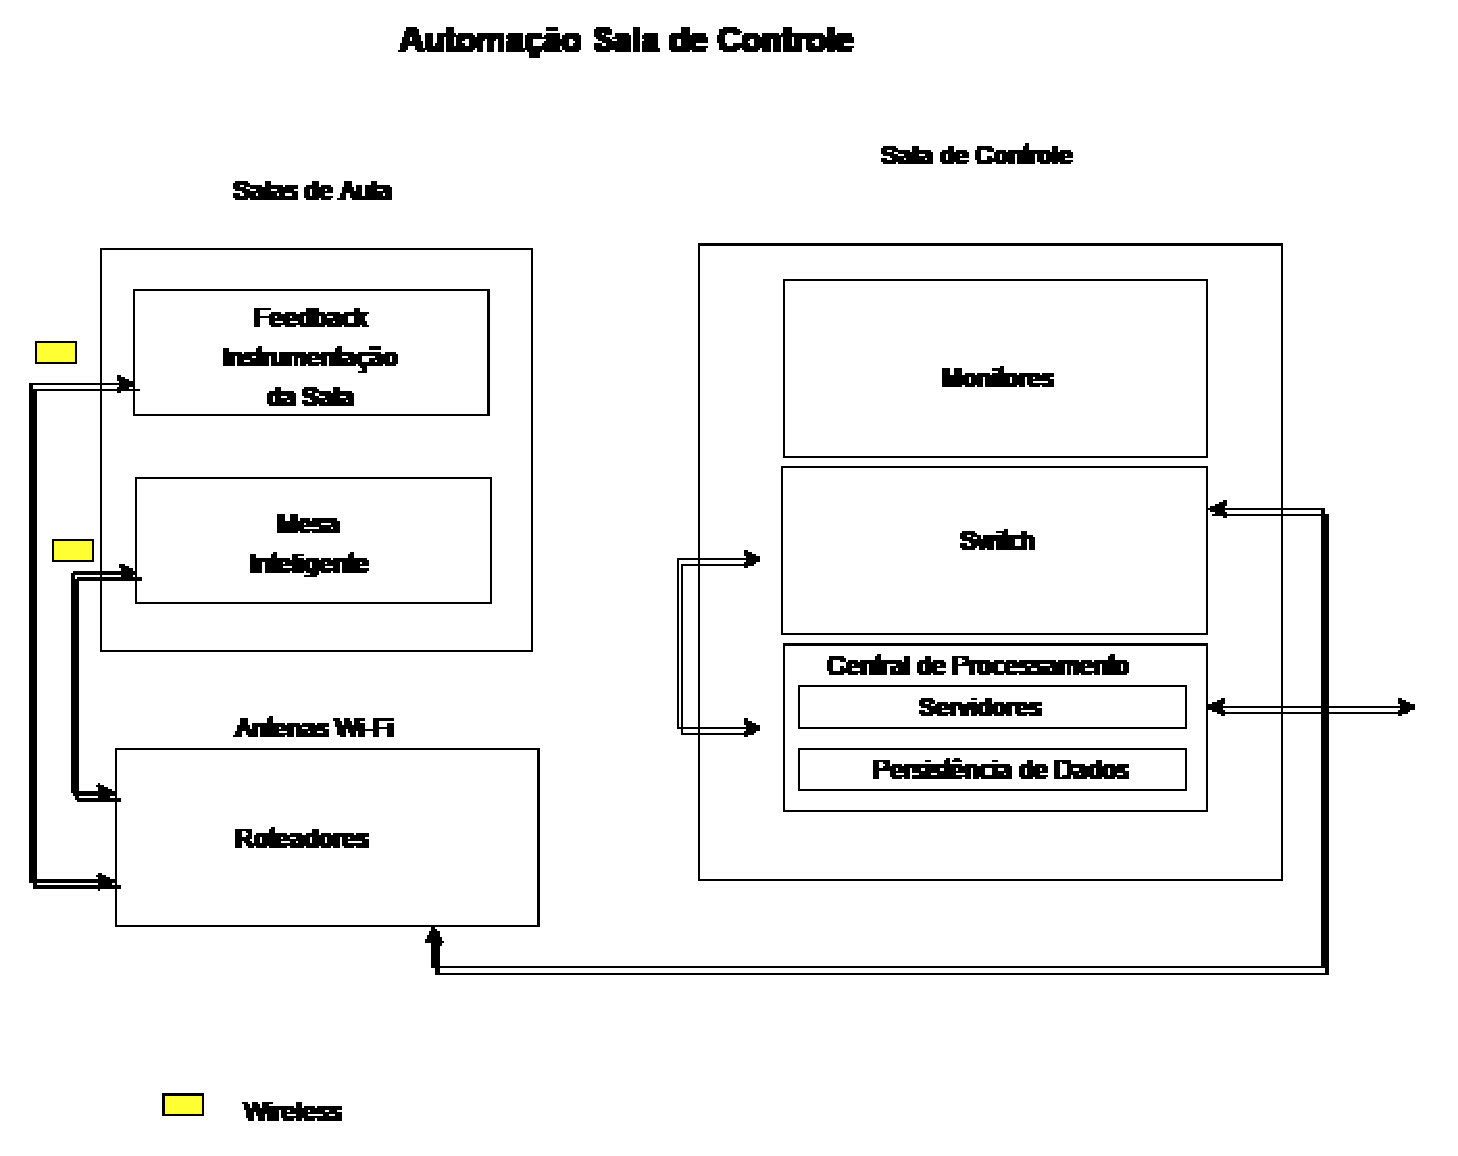
\includegraphics[keepaspectratio=true,scale=0.4]{figuras/automacao_sala_de_controle.eps}
  \caption{Sala de Controle}
  \label{fig:sala_cont}
\end{figure}

A conexão dos dispositivos com a sala de controle é representada nas figuras ~\ref{fig:plant_sup} e ~\ref{fig:plant_inf}. 

\begin{figure}[!h]
  \centering
  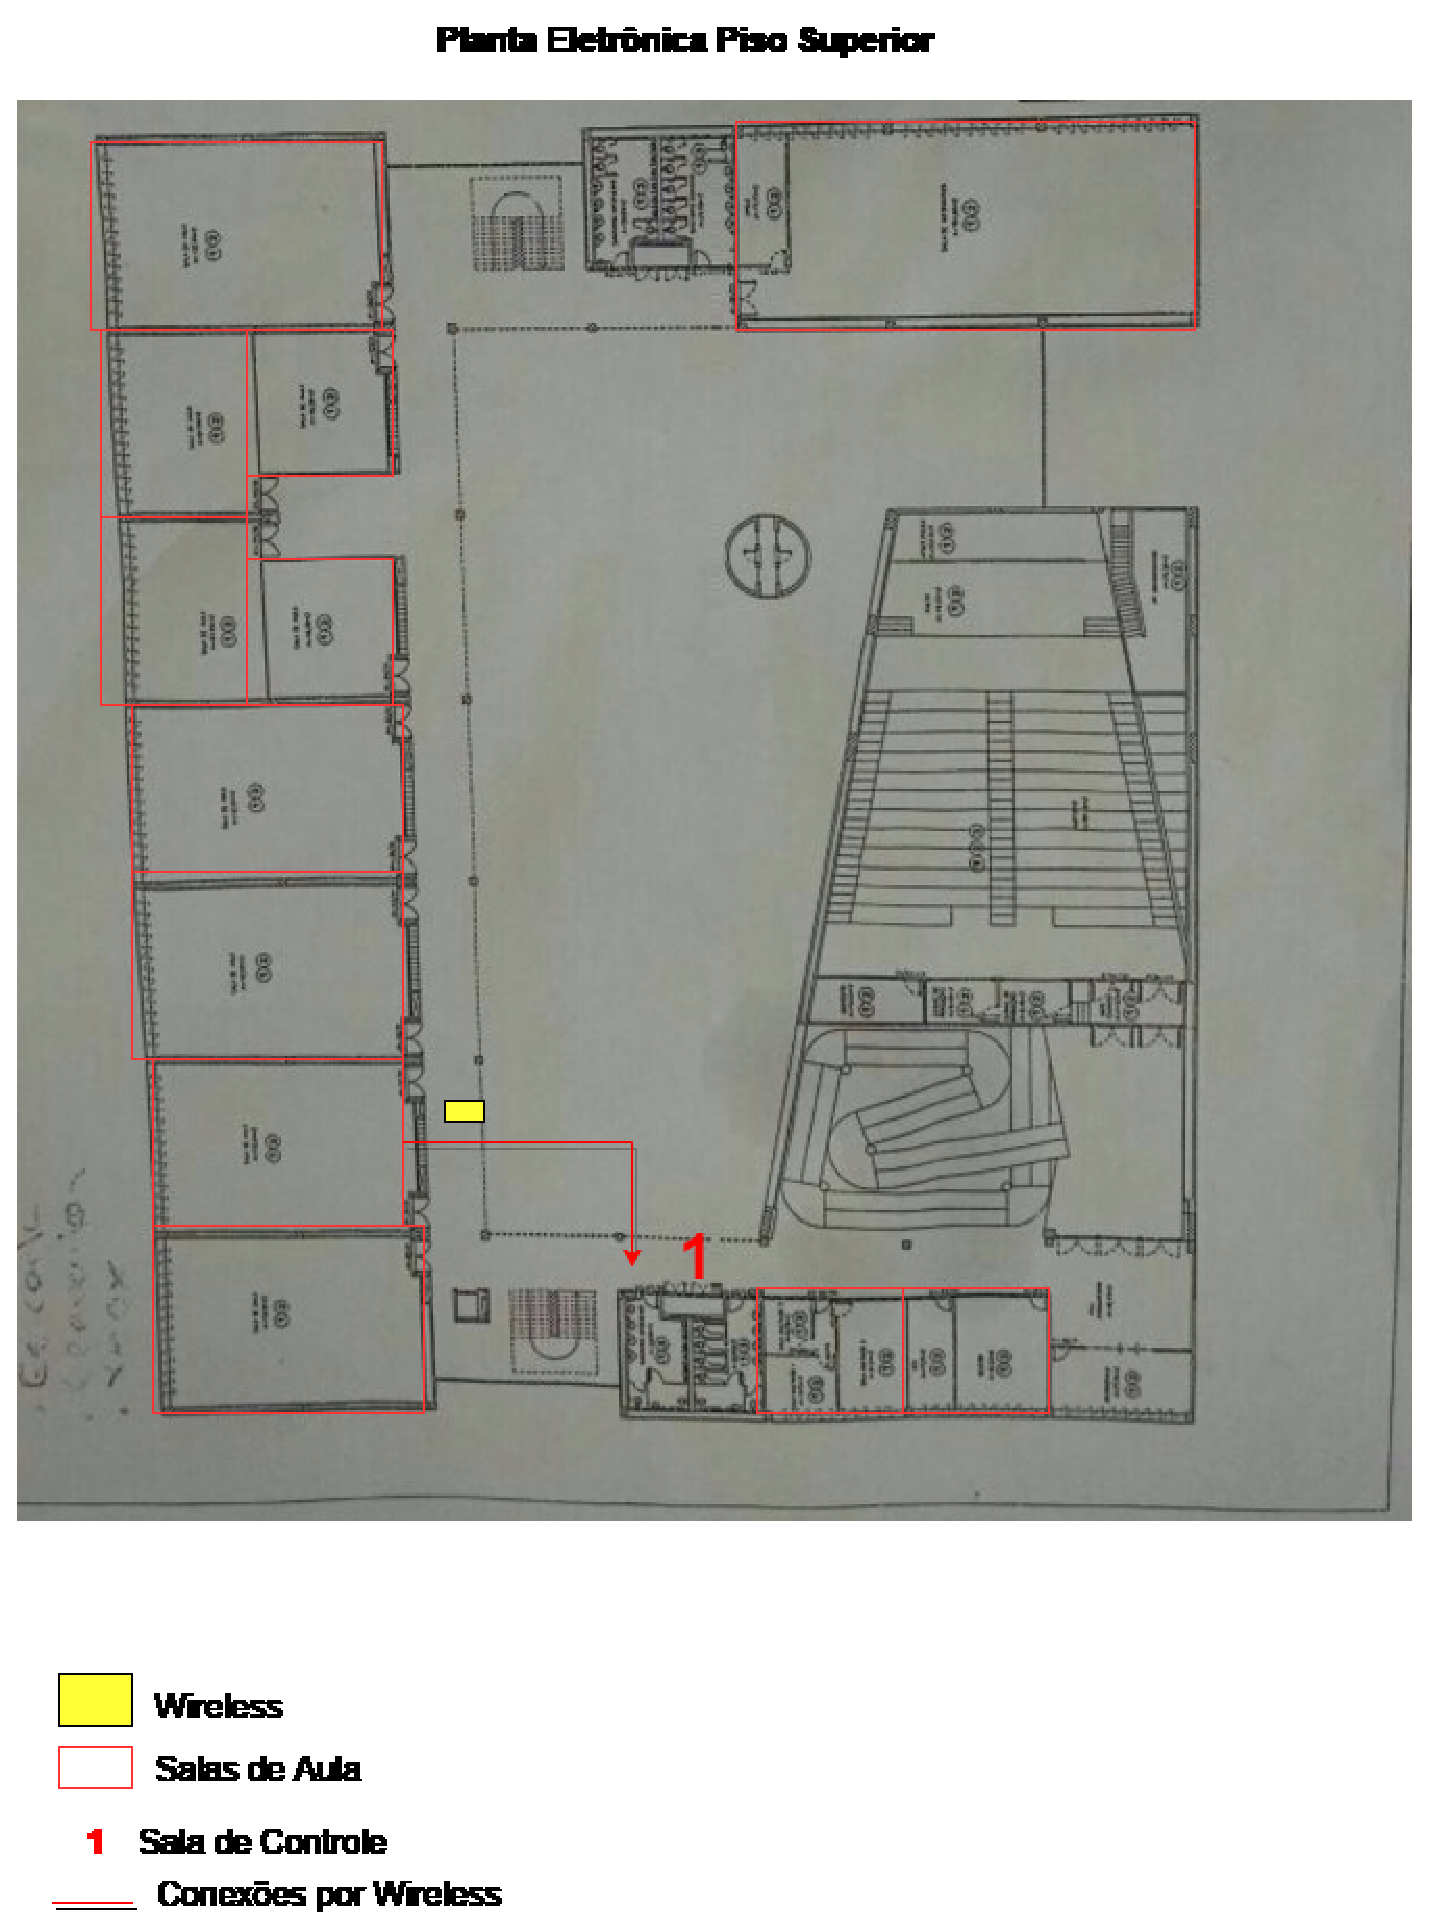
\includegraphics[keepaspectratio=true,scale=0.4]{figuras/planta_eletronica_superior.eps}
  \caption{Planta Eletrônica Piso Superior}
  \label{fig:plant_sup}
\end{figure}

\begin{figure}[!h]
  \centering
  \includegraphics[keepaspectratio=true,scale=0.3]{figuras/planta_eletronica_inferior.eps}
  \caption{Planta Eletrônica Piso Inferior}
  \label{fig:plant_inf}
\end{figure}

Além de enviar e receber dados da sala de controle, alguns dispositivos se comunicam uns com os outros, como no caso das salas de aula, onde a mesa inteligente controla todos os dispositivos de automação presentes nas salas, funcionando como um painel de controle central pada cada uma delas, como é mostrado nas figuras ~\ref{fig:sala_aula} e ~\ref{fig:sala_comp}.

\begin{figure}[!h]
  \centering
  \includegraphics[keepaspectratio=true,scale=0.3]{figuras/instrumentacao_da_sala.eps}
  \caption{Sala de Aula}
  \label{fig:sala_aula}
\end{figure}

\begin{figure}[!h]
  \centering
  \includegraphics[keepaspectratio=true,scale=0.3]{figuras/automacao_sala_de_computadores.eps}
  \caption{Sala de Computadores}
  \label{fig:sala_comp}
\end{figure}

\chapter[Interfaces e Processamento de Software]{Interfaces e Processamento de Software}
